\documentclass[twocolumn]{article}
\usepackage[top=1.1in, left=0.85in, right=0.85in]{geometry}

% \usepackage{eclbkbox}
\usepackage{amsmath}
\usepackage{amssymb}
\usepackage{code}
% \usepackage{amscd}
% \usepackage{xy}
\usepackage{graphicx}
% \usepackage{fancyhdr}
% \usepackage{color}
% \usepackage[dark,all,bottom,landscape,timestamp]{draftcopy}
% \usepackage{everypage}

% \pagestyle{empty}

% \usepackage{ulem}
% go back to italics for emphasis, though
% \normalem

\begin{document} 

\title{What words ought to exist? \\
       {\normalsize Coining with coinduction}}
\author{Dr.~Tom~Murphy~VII~Ph.D.\thanks{
Copyright \copyright\ 2011 the Regents of the Wikiplia
Foundation. Appears in SIGBOVIK 2011 with the blessing of the
Association for Computational Heresy; {\em IEEEEEE!} press,
Verlag-Verlag volume no.~0x40-2A.
\yen 0.00}
}


\renewcommand\>{$>$}
\newcommand\<{$<$}

\date{1 April 2011}

\maketitle

\begin{abstract}
This paper is an earnest attempt to answer the following question
scientifically: What words ought to exist?
\end{abstract}

\vspace{1em}
{\noindent \small {\bf Keywords}:
 computational cryptolexicography, n-Markov models, coinduction
}

\section*{Introduction}
During a recent high-stakes game of Scrabble-brand Crossword
Puzzle\footnote{Scrabble is a registered trademark of Hasbro
  Inc./Milton Bradley, and Mattel/JW Spear \& Sons plc.} I had what
could only be described as a killer bingo word (all 7 tiles) that,
after careful study, I determined could not be placed anywhere on the
board. Later in that same game, I had another sequence of letters that
just totally seemed like it should be able to make some long-ass
words, like for example ``oilsoap'' which turns out is not a legal
Scrabble word.\!\footnote{There are actually no 7-letter words that
  can be made from these letters. Don't even bother. Even if playing
  off an existing letter on the board, the best we can do are the
  non-bingos ``topsoil,'' ``topsail,'' or ``poloist'' with an
  available {\it t}.} This naturally made me frustrated and I wanted
to do something about it. Why can't ``oilsoap'' be a word? Or
``loopsia''? Words are introduced into the lexicon all the time. My
first reaction of course was to make an online version of Scrabble
where all words are legal. This is called Scrallbe (where they can
{\it all be} words!\footnote{As of 2011, the official Scrabble slogan
  is ``every word's a winner!'' which is clearly false.}) This is
available at {\tt http://snoot.org/toys/scrallbe}, and is pretty
boring, I gotta be honest (Figure~\ref{fig:scrallbe}).

\begin{figure}
\begin{center}
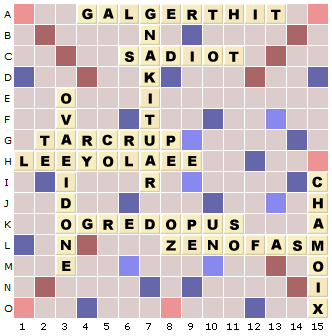
\includegraphics[width=0.75 \linewidth]{scrallbe-screenshot}
\end{center}\vspace{-0.1in}
\caption{In-progress Scrallbe game, 753 points.}
\label{fig:scrallbe}
\end{figure}

The thing is, it's just more fun when some words aren't words. Think
about it: If all words were real, then you could never make a really
devastatingly successful challenge in Scrabble that like, rocked the
whole household and turned a formerly casual family games night into
some kind of crying contest. Spelling bees could still exist, because
while no matter what those kids spelled,\!\footnote{Well, we have to
consider the possibility that the kiddo would use a letter that
doesn't exist. In this particular fantasy, grant me also that every
letter also exists, even $\stackrel{\Diamond}{\smile}$.} it would be
a word, it would not necessarily be the {\it right} word, just like
maybe a homophone. There would be fewer bar fights, but probably not
that many fewer. Moreover, iuhwueg nznie a uaohahweih zmbgba bawuyg!

Clearly we need more words, but not all of them. So this raises the
question: What words {\it ought} to exist? This paper explores several
different approaches for scientifically answering this question,
compares the results, and proposes specific words that should be
added, with their meanings.

Disclaimer possibly indicated for SIGBOVIK: The ``research'' contained
herein is 100\% legitimate.\!\footnote{Source code is available at
{\tt http://tom7misc.svn.
sourceforge.net/viewvc/tom7misc/trunk/wishlist/}} I have attempted to
present it in a tutorial style that assumes little mathematical or
computer science background. I have also left off the last {\it S} for
{\it Savings}.

\section{First idea: Wishlist}

My website ``{\sf snoot.org}'' has a number of games on it, including
a Scrabble clone called Scribble\footnote{{\tt
    http://snoot.org/toys/scribble/}} and Boggle clone called
Muddle.\!\footnote{{\tt http://snoot.org/toys/muddle/}} This website
has been running for almost ten years, comprising over 150,000
Scribble games totaling 3.8 million words placed and 628,000 Muddle
games with over 10 million words found. During each game, players
repeatedly attempt to play words that aren't real. The computer
rebukes them, but hope really springs eternal with these people. It's
like they truly deeply wish to break out of the shackles of the
Official Scrabble Players Dictionary.\!\footnote{For the analyses in
  this section that depend on a list of legal words, I actually use a
  modified version of SOWPODS, which is the tournament list used in
  Australia and the UK, and significantly more permissive than the US
  Tournament Word List. Though the modified version is non-canonical,
  I stuck with it because it's what's been in use on the site for
  ten years.} So the first approach to determining what
words ought to exist is to analyze the words that people tried to
play, in order to try to extract the essence of word-yearning.

This analysis is quite straightforward. I took the ten years of logs
files and extracted each attempt to play a word in Scribble or Muddle.
These log files are quite large, so the first step is just to get a
count, for each alleged word, and store those in a more convenient
format. There were 3,572,226 total words attempted\footnote{Here a
  word attempted is the major word of the play. This does not include
  incidental words (typically two-letter ones) formed in the
  perpendicular direction.} in Scribble and 13,727,511 in Muddle. The
most frequent ones appear in Figure~\ref{fig:mostfrequent}. Aside from
the one-letter ones, the most frequent words are legitimate words,
since players have a bias towards attempting words that will not be
rebuked by the computer.

Seeing the words that people wish existed is a simple matter of
filtering out the words that already exist, using the Scrabble
dictionary. (I also filtered out one-letter ``words''. It is easy to
see that no one-letter words should exist, again because of
ambiguities created in spelling bees. Not only when literally spelling
``bees'', but according to the official Scripps National Spelling Bee
rules, the speller may optionally pronounce the word to be spelled
before and after spelling it. So if ``s'' were a word, then the
following ridiculous exchange obtains: Judge: ``S. The letter {\it s}.
Etruscan origin.'' Speller: ``S. S. S.'' and the judge cannot tell if
the speller meant to state the word before and after, or thinks the
word is spelled ``sss''.) 22.3\% of the words attempted in Scribble
and 36.8\% in Muddle were not real. The most frequent ones appear in
Figure~\ref{fig:mostfrequentfake}.

\begin{figure}
\begin{center}
\begin{tabular}{|rl@{\qquad}rl|}
\multicolumn{2}{l}{{\bf \large Scribble}} &
\multicolumn{2}{l}{{\bf \large Muddle}} \\
\hline
Count & Word & Count & Word \\
\hline
45,605  &  a        &     20,412  &  late  \\
42,315  &  i        &     19,405  &  rate  \\
32,499  &  d$^*$    &     19,276  &  dear  \\
12,981  &  in       &     19,049  &  tear  \\
12,851  &  oe       &     19,019  &  date  \\
12,528  &  s$^*$    &     18,771  &  lear  \\
12,207  &  re       &     18,423  &  deal  \\
11,159  &  tv       &     18,231  &  real  \\
10,720  &  jo       &     18,138  &  lead  \\
10,386  &  it       &     18,076  &  tale  \\
10,369  &  et       &     17,969  &  lane  \\
9,659   &  qua      &     17,956  &  sear  \\
9,218   &  xi       &     17,570  &  read  \\
9,099   &  go       &     17,193  &  teal  \\
9,052   &  ow       &     17,170  &  lean  \\
8,801   &  qat      &     17,071  &  dare  \\
8,602   &  aa       &     16,923  &  dale  \\
8,278   &  un       &     16,892  &  seal  \\
8,142   &  en       &     16,806  &  sale  \\
8,005   &  or       &     16,465  &  seat  \\
\hline
\end{tabular}
\end{center}
\caption{Most frequently attempted words in Scribble and Muddle. Asterisks
indicate non-words.}
\label{fig:mostfrequent}
\end{figure}

\begin{figure}
\begin{center}
\begin{tabular}{|rl@{\qquad}rl|}
\multicolumn{2}{l}{{\bf \large Scribble}} &
\multicolumn{2}{l}{{\bf \large Muddle}} \\
\hline
Count & Word & Count & Word \\
\hline
11,159 &  tv         &     16,251 &  dane    \\
4,003  &  ok         &     6,156  &  rane    \\
2,862  &  iraq       &     5,603  &  sare    \\
2,725  &  zen        &     5,576  &  nate    \\
2,448  &  cho        &     4,863  &  mear    \\
1,538  &  viz        &     4,750  &  cale    \\
1,418  &  sdasda     &     4,616  &  nees    \\
1,396  &  von        &     4,568  &  nale    \\
1,136  &  etc        &     4,507  &  fale    \\
878    &  int        &     4,347  &  deat    \\
829    &  june       &     4,263  &  tean    \\
745    &  lp         &     4,251  &  nile    \\
719    &  zion       &     4,160  &  mens    \\
665    &  cia        &     4,087  &  deel    \\
661    &  jim        &     3,851  &  deam    \\
651    &  iraqi      &     3,828  &  dana    \\
648    &  ques       &     3,781  &  beed    \\
542    &  que        &     3,769  &  lans    \\
502    &  tim        &     3,725  &  tade    \\
\hline
\end{tabular}
\end{center}
\caption{Most frequently attempted non-words in Scrabble and Muddle.}
\label{fig:mostfrequentfake}
\end{figure}

There's a clear difference between these two lists. The Scribble list
is dominated by words involving difficult-to-play letters like {\it v}
(there are no legal two-letter {\it v}-words). Most of the words would
probably be acknowledged as real, just not legal in Scribble. The ones
that don't already have meanings, like ``cho'' and ``int'' and ``que''
seem to be pretty good candidates to exist. The Muddle list is all
four-letter words (the minimum allowed length) using common letters.
Other than the ones that are already words, like ``dane'' and ``nile''
and ``mens'' (as in ``mens section'' or ``the powerfuel weapon kills
hard so many mens''), these are all good candidates for words to
exist. Probably if you were playing someone really intense in
Scrabble, and he or she played one of these, and was super deadpan
about it and maybe had caused some crying contests before, and a known
sesquipedalianist, you would let these fly because they look like real
words to me. A point in their favor is that they would be quite
low-scoring words in Scrabble; not a {\it z} or {\it q} to be found.
Even in the Scribble list there's no ``qzkwv'' junk. The effect is
probably due to a few factors: Players are less likely to attempt
obvious non-words, common letters appear more often on the rack and on
the board and so the opportunity to play words like in
Figure~\ref{fig:mostfrequentfake} presents itself more frequently, and
in Muddle, there is no advantage to using unusual letters, except the
joy of being a weirdo. Nonetheless, these lists are surely biased by
the specifics of Scribble and Muddle, and the question at hand is not
just what words ought to exist for the purpose of internet word games,
but for general purposes.

\begin{figure}[t]
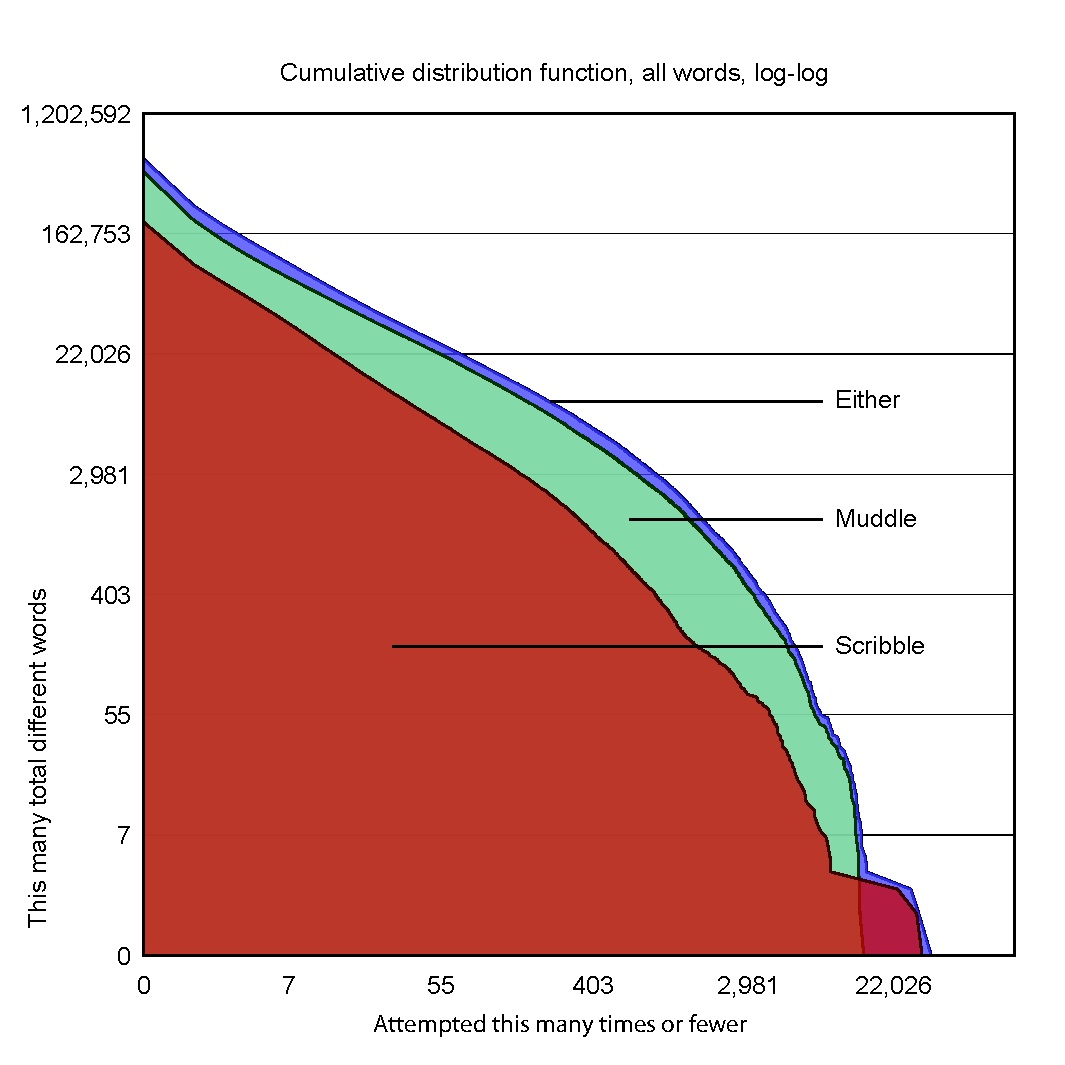
\includegraphics[width=\linewidth]{wishlist-cdf}
\vspace{-0.1in}\caption{Cumulative distribution of word frequency.
  Approximately 25,000 different words (y axis) were issued 55 times
  or fewer (x axis). The ``total'' area does not appear much larger
  than its components because this is a log-log plot.}
\label{fig:gamedistribution}
\end{figure}

Another downside is that this method completely ignores the many words
that are attempted only once or a small number of times. Players are
very creative; of the 564,610 unique words attempted, 501,939 of them
aren't real! The vast majority of words are attempted only a handful
of times (Figure~\ref{fig:gamedistribution}). Though those words
individually are not good candidates to exist, like tiny stars wished
upon in the night sky,\!\footnote{Astronomers now agree that stars do
  exist, by the way.} in aggregate they form a significant planetarium
that may tell us what {\it kind} of words people wish existed. For
example, if we saw that the words ``sweeeeeeet'',
``sweeeeeeeeeeeeet'', ``sweeeet'' and ``sweeeeeeeeeeeeeet'' occurred a
few times each, we could infer that people wished that words like
``sweet'' with strictly more than two {\it e}s were real words. They
might even be indifferent to the absolute number of {\it e}s, as long
as there existed some legal variation with more than two {\it e}s.
(This appears to be borne out by data. According to Google's
estimates, the words ``swe$^n$t'' for various medium-sized $n$
(10--20) appear on the Internet with similar frequency. The only
exception is ``sweeeeeeeeeeeeeeeeeeet'', with 19 {\it e}s, which
unexpectedly appears three times as often as 18 or 20 {\it e}s does;
see Figure~\ref{fig:sweet}.) In order to lance these two boils, in the
next section I explore statistical methods for generalizing from lots
of individual examples.

% XXX should really try to get this in the right column, since it
% overflows the margins
\begin{figure}
\begin{tabular}{r|r|l}
17,900,000 & 0 & swt \\
1,060,000 & 1 & swet \\
580,000,000 & 2 & sweet \\
1,310,000 & 3 & sweeet \\
806,000 & 4 & sweeeet \\
509,000 & 5 & sweeeeet \\
283,000$^1$ & 6 & sweeeeeet \\  % spell correction for five
170,000 & 7 & sweeeeeeet \\
115,000 & 8 & sweeeeeeeet \\
75,200 & 9 &  sweeeeeeeeet \\
94,300$^2$ & 10 & sweeeeeeeeeet \\ % spell correction for nine?
51,700 & 11 & sweeeeeeeeeeet \\
37,900 & 12 & sweeeeeeeeeeeet \\
32,000 & 13 & sweeeeeeeeeeeeet \\
25,300 & 14 & sweeeeeeeeeeeeeet \\
24,300 & 15 & sweeeeeeeeeeeeeeet \\
41,000$^3$ & 16 & sweeeeeeeeeeeeeeeet \\ % spell correction for 14
55,000 & 17 & sweeeeeeeeeeeeeeeeet \\
45,000 & 18 & sweeeeeeeeeeeeeeeeeet \\
133,000$^4$ & 19 & sweeeeeeeeeeeeeeeeeeet \\ % for 15
34,800 & 20 &  sweeeeeeeeeeeeeeeeeeeet \\
%
16,100$^5$ & 25 & sweeeeeeeeeeeeeeeeeeeeeeeeet \\ % for weeeeeeeeeeeeeeeeeeeeeeeee t
10,100 & 30 & sweeeeeeeeeeeeeeeeeeeeeeeeee\ldots t \\
2,800 & 40 &  sweeeeeeeeeeeeeeeeeeeeeeeeee\ldots t \\
923 & 50 &    sweeeeeeeeeeeeeeeeeeeeeeeeee\ldots t \\
118 & 75 &    sweeeeeeeeeeeeeeeeeeeeeeeeee\ldots t \\
38 & 100 &    sweeeeeeeeeeeeeeeeeeeeeeeeee\ldots t  \\
?$^6$ & 200 & sweeeeeeeeeeeeeeeeeeeeeeeeee\ldots t     \\ % word is too long for Google
\end{tabular}
\caption{Frequency of ``swe$^n$t'' on the internet for various $n$, estimated
by Google. Notes: {\bf (1)} Spell correction offered for ``sweeeeet''. {\bf (2, 3, 4)} Spell corrections
offered to e$^{9}$, e$^{14}$ and e$^{15}$ respectively. {\bf (5)} Spell correction offered for ``weeeeeeeeeeeeeeeeeeeeeeeee t'' (?) {\bf (6)} With two hundred {\it e}s, the word is too long for Google, which asks me to ``try using a shorter word.'' Thanks Google, but I already did try the shorter ones.}
\label{fig:sweet}
\end{figure}

\section{Statistical models}

The reason that people are more likely to play words like ``rane'' is
that the letters are common---they appear more often in words, and
more often in the Scrabble bag. But it's not simply a matter of the
frequency of letters; if it were, we would expect to see words like
``eee'' dominating the list, since {\it e} is the most common letter
in English.\!\footnote{Tied for first place with {\it n}, {\it g},
{\it l}, {\it i}, {\it s}, and {\it h}.} People do not play such words
often because they do not {\it seem} like real words. ``oilsoap''
seems more like a word than ``ioaopsl'' to most non-crazy people,
even though they contain the same letters. This is because we have
expectations on what letters are likely to appear next to one
another in words. This section is about modeling expectations on
what letters appear together, and then using that model to generate
the most likely words that don't yet exist.

{\bf Markov chains.}\,
This guy called Andrei Markov had an idea which is pretty obvious in
retrospect, but he had it like a hundred years ago before any of us
were born (probably; if not: you are old), which he didn't call Markov
chains but now they're called Markov chains because I guess in the
hopes that contemporary mathematicians will get stuff named after
their dead selves if they keep the tradition of naming stuff after
dead people alive. The idea is easiest to understand in the context
of the current problem. Suppose we know that the words ``hello'',
``helpful'' and ``felafel'' are the only real words. The following
is a frequency table of how often each letter occurs.

\begin{center}
\begin{tabular}{|r|r|r|r|r|r|r|r|} % {helopfua}
\hline
h   & e   & l   & o   & p   & f   & u   & a    \\
\hline
2   & 4   & 6   & 1   & 1   & 3   & 1   & 1    \\
\hline
\end{tabular}
\end{center}

This tells us that {\it l} is by far the most common letter, so the
most likely word is probably ``l'' or ``llllllll'' or something. A
Markov chain is like a frequency table, but instead of counting
individual letters, we count how often one letter comes {\it after}
another. Here is the Markov chain for those words.

% of the current problem. Suppose we know that the words ``hello'',
% ``helpful'' and ``felafel'' are the only real words. The following

\begin{center}
\begin{tabular}{|c|r|r|r|r|r|r|r|r|} % {helopfua}
\hline
\,  &  {\bf h}   & {\bf e}   & {\bf l}   & {\bf o}   & {\bf p}   & {\bf f}   & {\bf u}   & {\bf a} \\
\hline  %    h     e     l     o     p     f     u     a
{\bf h}   &  0   & 0   & 0   & 0   & 0   & 0   & 0   & 0    \\
\hline
{\bf e}   &  2   & 0   & 0   & 0   & 0   & 2   & 0   & 0    \\
\hline
{\bf l}   &  0   & 4   & 1   & 0   & 0   & 0   & 1   & 0    \\
\hline
{\bf o}   &  0   & 0   & 1   & 0   & 0   & 0   & 0   & 0    \\
\hline
{\bf p}   &  0   & 0   & 1   & 0   & 0   & 0   & 0   & 0    \\
\hline
{\bf f}   &  0   & 0   & 0   & 0   & 1   & 0   & 0   & 1    \\
\hline
{\bf u}   &  0   & 0   & 0   & 0   & 0   & 1   & 0   & 0    \\
\hline
{\bf a}   &  0   & 0   & 1   & 0   & 0   & 0   & 0   & 0    \\
\hline
\end{tabular}
\end{center}

The letters across the top are the ``previous letter'' and the ones
across the left are the ``next letter'' and the box contains the
corresponding count. For example, the pair ``el'' appears four times.
(Pairs of letters are called ``bigrams'' by nerds, some nerd-poseurs,
and Markov who I can't tell if he was a nerd by his picture, because
he does have a pretty austere beard, but also did a lot of math.) One
of the useful things about a Markov chain is that it lets us predict
the next letter that we might see. For example, if we see ``half'',
then the column labeled {\bf f} above tells us that the next letter is
twice as often an {\it e} than a {\it u}, and that no other letters
ever occurred. Typically we think of these as being probabilities
inferred from our observations, so we say there's a 2/3 chance of {\it
e} following {\it f} and a 1/3 chance of {\it u}. Now the word ``llllll''
isn't so likely any more, because there's only a 1/4 chance of the
next letter being {\it l} once we see {\it l}.

Words are not just their interiors; it's also important what letters
tend to start and end words. We can do this by imagining that each
word starts and ends with some fake letters, and include those in the
Markov chain. Let's use {\bf \<} for the start symbol and {\bf \>} for
the end. So we pretend we observed ``\<hello\>'', ``\<helpful\>'', and
``\<felafel\>''. Speaking of which, could you imagine if there were such
a thing as a helpful felafel? Would you eat it? Because then it
probably can't help you any more, except to get fat.

\begin{center}
\begin{tabular}{|c|r|r|r|r|r|r|r|r|r|} % {helopfua}
\hline
\,  &  {\bf \<}    & {\bf h}   & {\bf e}   & {\bf l}   & {\bf o}   & {\bf p}   & {\bf f}   & {\bf u}   & {\bf a}    \\
\hline  %  \<     h     e     l     o     p     f     u     a
{\bf h} &  2  &  0   & 0   & 0   & 0   & 0   & 0   & 0   & 0    \\
\hline    
{\bf e} &  0  &  2   & 0   & 0   & 0   & 0   & 2   & 0   & 0    \\
\hline    
{\bf l} &  0  &  0   & 4   & 1   & 0   & 0   & 0   & 1   & 0    \\
\hline    
{\bf o} &  0  &  0   & 0   & 1   & 0   & 0   & 0   & 0   & 0    \\
\hline    
{\bf p} &  0  &  0   & 0   & 1   & 0   & 0   & 0   & 0   & 0    \\
\hline    
{\bf f} &  1  &  0   & 0   & 0   & 0   & 1   & 0   & 0   & 1    \\
\hline    
{\bf u} &  0  &  0   & 0   & 0   & 0   & 0   & 1   & 0   & 0    \\
\hline    
{\bf a} &  0  &  0   & 0   & 1   & 0   & 0   & 0   & 0   & 0    \\
\hline    
{\bf \>} &  0  &  0   & 0   & 2   & 1   & 0   & 0   & 0   & 0    \\
\hline
\end{tabular}
\end{center}

We just added these like other letters, but since the beginning symbol
{\bf \<} never occurs after other letters, we don't need a row for it
(it would be all zeroes), and similarly since no letters ever follow
{\bf \>} we don't need a column for it. Now the word ``lllll'' is
impossible because no words start with {\it l}.

It basically makes sense to consider the probability of a whole word
to be the chance of simultaneously seeing each pair of letters in it,
which is just the product of all the probabilities. So the word
``hel'' is $2/3$ (for {\bf \<h}) $\times$ 2/2 (for {\bf he}) $\times$
4/4 (for {\bf el}) $\times$ 2/6 (for {\bf l\>}), which is $0.222$.
These are the most likely words overall (I discuss how to generate
such lists in Section~\ref{sec:coin}):

\begin{center}
\begin{tabular}{rl@{\quad\quad}rl}
22.2\%  &  hel      &      2.5\%  &  helpfel  \\
11.1\%  &  helo     &      2.5\%  &  helafel  \\
 7.4\%  &  fel      &      1.9\%  &  fulo     \\
 3.7\%  &  hell     &      1.9\%  &  hello    \\
 3.7\%  &  felo     &      1.2\%  &  fell     \\
 3.7\%  &  ful      &      1.2\%  &  helafelo \\
\end{tabular}
\end{center}

This is pretty good. These words resemble the ones we observed to build
the Markov chain, but are novel. I think helafelo is a pretty rad word,
right?

\begin{figure}[t]
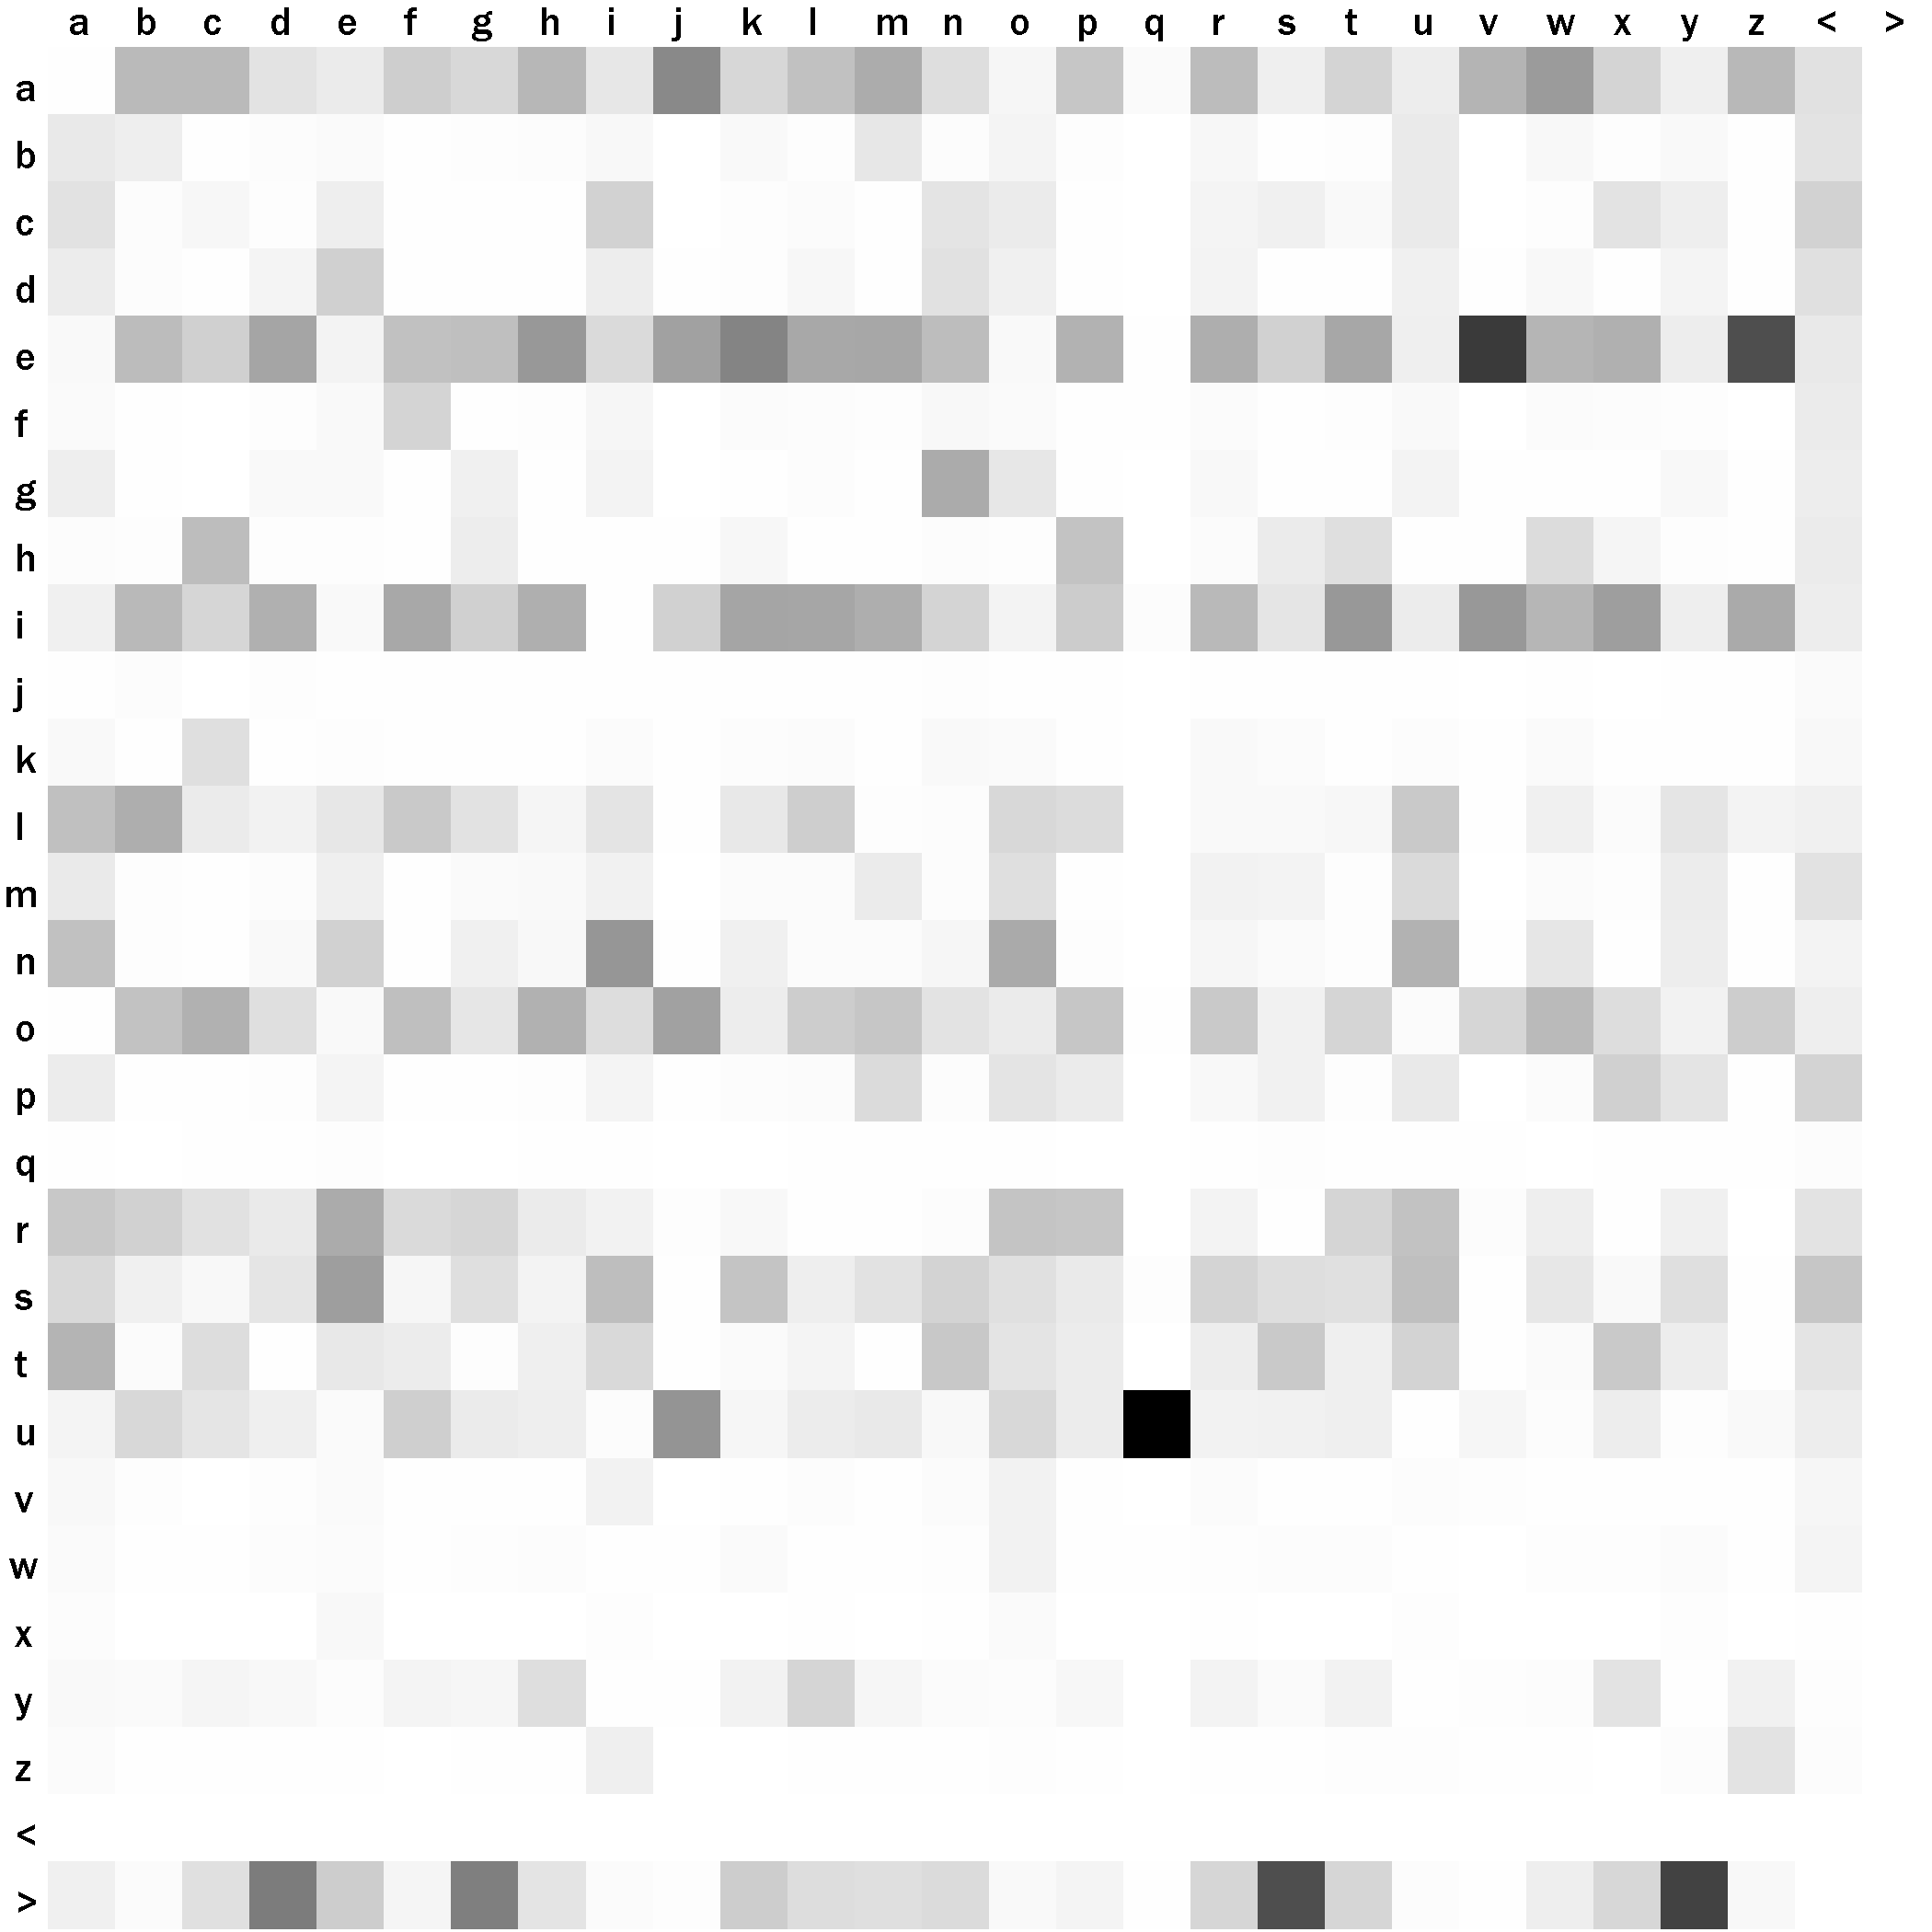
\includegraphics[width=\linewidth]{coin1}
\caption{Markov chain for the SOWPODS word list, where darker squares
indicate higher probability. The darkest is the transition from {\it q}
to {\it u} ($98\%$), which is not surprising.}
\label{fig:sowpodsbigrams}
\end{figure}

The next step is to build a Markov chain for a list of real words and
see what results. I built one for the SOWPODS word list, which results
in the table in Figure~\ref{fig:sowpodsbigrams}. These
are the most likely words, with real words filtered out:

% XXX improve layout
\begin{center}
\begin{tabular}{rl@{\quad\quad}rl}
4.99\%  & s     &   0.17\%  & y   \\
1.75\%  & d     &   0.17\%  & p   \\
0.95\%  & g     &   0.16\%  & a   \\
0.55\%  & c     &   0.16\%  & n   \\
0.43\%  & r     &   0.15\%  & ps  \\
0.42\%  & t     &   0.13\%  & ms  \\
0.40\%  & e     &   0.13\%  & ts  \\
0.35\%  & m     &   0.13\%  & ds  \\
0.32\%  & ss    &   0.11\%  & hy  \\
0.20\%  & rs    &   0.11\%  & k   \\
0.19\%  & h     &   0.11\%  & ng  \\
0.18\%  & l     &   0.11\%  & ly  \\
\end{tabular}
\end{center}


Ugh, poop city! Actually, it turns out that when you see enough words,
you see enough pairs that all sorts of junk looks likely. For example,
``ng'' is easily explained by many words starting with {\it n}, {\it
g} often following {\it n}, and many words ending with {\it g}. Even
though each pair makes sense, the whole thing doesn't look like a word,
because we expect to at least see a vowel at some point, for one thing.

There is a standard solution to this problem, which is to generalize
the Markov chain to keep more than one letter of history. So instead
of just tallying how often {\it g} follows {\it n}, we count how often
{\it g} follows {\it in} (and any other pair of letters).\!\footnote{
  The details are straightforward, except possibly that we now imagine
  each word to start with two (or in general, $n$) copies of the start
  symbol, so that we see ``\<\<helpful\>''. The column corresponding
  to the history {\bf \<\<} tells us the frequency of letters that
  start words, and for example the column {\bf \<h} tells us the
  frequency of letters that follow {\it h} when it appears at the
  start of a word. We do not need to repeat the ending character \>
  because once we see it, we never do anything but end the word.} This
makes the table pretty large, so you'll just have to look at
Figure~\ref{fig:sowpodsbigrams} again and imagine it being 28 times
wider. But the good news is that it invents much better words:

\begin{center}
\begin{tabular}{rl@{\quad\quad}rl}
\multicolumn{4}{c}{Markov chain with $n=2$.} \\
\hline
.709\% & ing     &   .110\% & le    \\
.248\% & ses     &   .107\% & der   \\
.169\% & des     &   .107\% & ove   \\
.154\% & nes     &   .101\% & gly   \\
.140\% & sts     &   .088\% & hy    \\
.131\% & se      &   .085\% & ung   \\
.128\% & ings    &   .083\% & cy    \\
.126\% & ded     &   .081\% & pres  \\
.117\% & cal     &   .080\% & pers  \\
\end{tabular}
\end{center}

These are even, like, pronounceable. The best news is that they keep
getting better the more history we keep:

\begin{center}
\begin{tabular}{rl@{\quad\quad}rl}
\multicolumn{4}{c}{Markov chain with $n=3$.} \\
\hline
.109\% & des     &   .038\%  & ent     \\
.078\% & pers    &   .036\%  & dist    \\
.076\% & cal     &   .035\%  & ble     \\
.062\% & pres    &   .035\%  & ches    \\
.045\% & nons    &   .034\%  & gly     \\
.044\% & ress    &   .034\%  & inted   \\
.042\% & ing     &   .034\%  & dists   \\
.040\% & pred    &   .033\%  & lity    \\
\end{tabular}
\end{center}


\begin{center}
\begin{tabular}{rl@{\quad\quad}rl}
\multicolumn{4}{c}{Markov chain with $n=4$.} \\
\hline
.045\% & unders  &   .017\% & heters  \\
.034\% & dising  &   .016\% & sters   \\
.029\% & pers    &   .015\% & stic    \\
.028\% & cally   &   .014\% & pering  \\
.023\% & inted   &   .013\% & dises   \\
.020\% & heter   &   .013\% & ching   \\
.019\% & tric    &   .012\% & shing   \\
.018\% & ster    &   .012\% & dest    \\
.018\% & hier    &   .011\% & teless  \\
.018\% & unded   &   .011\% & resis   \\
\end{tabular}
\end{center}

\begin{center}
\begin{tabular}{rl@{\quad\quad}rl}
\multicolumn{4}{c}{Markov chain with $n=5$.} \\
\hline
\multicolumn{4}{l}{{\tt GetTempFileName failed with error 5}} \\
\end{tabular}
\end{center}

With four letters of history, the words produced are quite good! (The
results at $n=5$ are somewhat disappointing since the program crashes
from running out of memory. The table at $n=5$ would have over 481
million entries.) Many of these seem like real words. Some even
suggest meaning because they contain common morphemes. To make the
case that these are not just real-looking words but characteristic of
the English language, compare the results of the same algorithm on the
dictionary from the Italian language edition of Scrabble, which is
probably called {\it Scrabblizzimo!} (Figure~\ref{fig:italian}).
Italian is lexicographically a more compact language than English
(Figure~\ref{fig:italianbigrams}); there are only 21 letters (outside
of occasional interlopers in loan words like {\it jeans} and {\it
  taxi}). Moreover, even though the dictionary contains 585,000 words
(twice as many as English), the probabilities of observing these
non-words are much higher than the most likely English ones.

\begin{figure}[t]
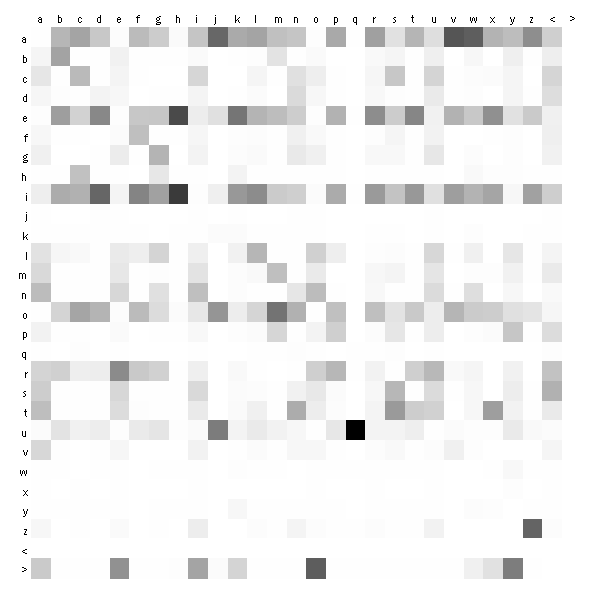
\includegraphics[width=\linewidth]{italiancoin1}
\caption{Markov chain for the Italian language. Again darker cells
  indicate higher probability. Italian has more lexicographic
  structure recognizable from bigraphs than English does: Note that
  the extremely rare letters ``j'', ``k'', ``q'', ``w'', ``x'', and
  ``y'' have almost empty rows. ``z'' very frequently follows ``z'',
  as in {\it pizza}. Words almost always end in a vowel.}
\label{fig:italianbigrams}
\end{figure}

\begin{figure}
\begin{center}
\begin{tabular}{rl@{\quad\quad}rl}
.137\%  &  ammo       &   .026\%  &  rino      \\
.071\%  &  rice       &   .025\%  &  diste     \\
.061\%  &  rico       &   .024\%  &  risti     \\
.055\%  &  este       &   .023\%  &  disci     \\
.053\%  &  scono      &   .022\%  &  riasse    \\
.049\%  &  immo       &   .022\%  &  riassi    \\
.047\%  &  assero     &   .021\%  &  cate      \\
.047\%  &  scano      &   .019\%  &  rite      \\
.038\%  &  rammo      &   .019\%  &  cando     \\
.034\%  &  cata       &   .018\%  &  riassero  \\
.034\%  &  assimo     &   .018\%  &  riassimo  \\
.032\%  &  riate      &   .018\%  &  dete      \\
.032\%  &  disce      &   .018\%  &  disca     \\
.030\%  &  esti       &   .017\%  &  risca     \\
.029\%  &  rica       &   .017\%  &  cente     \\
.028\%  &  endo       &   .016\%  &  acci      \\
.027\%  &  dissimo    &   .015\%  &  centi     \\
.026\%  &  rici       &   .015\%  &  girono    \\
\end{tabular}
\end{center}
\caption{Most probable words induced by the Markov Markov chain for
  the Italian language ($n=4$).}
\label{fig:italian}
\end{figure}


\subsection{Usage-weighted methods}

One criticism of this approach is that it considers every word in the
word list to be equally important.\!\footnote{In fact, the common part
  of words with many different conjugations is in essence counted many
  times. This means {\it ornithology} in its six different forms
  contributes six times as much to our model as the word {\it the}!} I
object on the philosophical grounds that some words that already exist
{\em ought to exist more} than other words that already exist. For
example, {\it congenital} is a much nicer word than the plain ugly
{\it congenial}, and is reflected by the fact that {\it congenital} is
used five times more frequently than {\it
  congenial}.\!\footnote{14,200,000 times to 2,820,000, on the
  Internet, according to Google.} In this section, we produce Markov
models of words weighted by the frequency with which people tend to
use them. This is just a simple matter of training the model on some
natural language corpus (with many occurrences of each word, or no
occurrences of unpopular words) rather than a flat list of all alleged
words.

{\bf Facebook.}\ Since the best research is intensely navel-gazing, I started by 
analyzing a corpus of my own writing, specifically my Facebook status
updates since March~2006. There were 1,386 status updates containing
such gems as ``Tom Murphy VII thinks mathfrak is straight ballin''
and ``Tom Murphy VII global L\_50 reused for unused\_36166!!''. The
most likely words with $n=4$:

\begin{center}
\begin{tabular}{rl@{\quad\quad}rl}
\multicolumn{4}{c}{My Facebook status updates, $n=4$.} \\
\hline
.252\% &  pittsburgh   & .097\% &  can't    \\   
.209\% &  steelers     & .083\% &  i'm      \\   
.209\% &  sfo          & .083\% &  icfp     \\   
.195\% &  it's         & .083\% &  app      \\   
.125\% &  bdl          & .069\% &  x        \\   
.111\% &  sigbovik     & .069\% &  drunj    \\   
.109\% &  facebook     & .069\% &  g        \\   
.097\% &  mic          & .061\% &  ther     \\   
.097\% &  s            & .055\% &  doesn't  \\
\end{tabular}
\end{center}

This is the worst. Not only does it contain loads of one-letter words that
we have already determined are verboten,\!\footnote{Note that since $n=4$ these
words have to actually appear in status updates to have nonzero probability for
this list. ``g'' is explained by frequent occurrences of ``e.g.'', for example.}
but the rest are just non-words that I tend to use like the names of cities,
prestigious conferences, or IATA airport codes. The main problem is that there
is simply not enough data from which to generalize.

{\bf Wikipedia.}\ I tried again, but with Wikipedia, using a snapshot
of the English site from June~2009. This is 23 gigabytes of data, most
of it expository text composed by native speakers, plus bathroom humor
vandalism. The list produced by this analysis is much better, though it
contains artifacts from non-English Wiki language used in articles. The
unabridged list appears in the appendix; my hand-selected favorites:

\begin{center}
\begin{tabular}{rl@{\quad\quad}rl}
\multicolumn{4}{c}{English Wikipedia, $n=3$.}     \\
\hline
.0287\% & smally      &     .00518\% & reporth    \\
.0156\% & websity     &     .00484\% & delection  \\
.0156\% & stude       &     .00459\% & grounty    \\
.0124\% & chool       &     .00437\% & betweek    \\
.0120\% & fontry      &     .00431\% & fination   \\
.0102\% & undex       &     .00388\% & manuary    \\
.0099\% & octory      &     .00360\% & whicle     \\
.0096\% & coibot      &     .00262\% & stategory  \\
.0084\% & footnot     &                           \\
\end{tabular}
\end{center}


Lots of these could be the names of tech startups or Pok\'emon.

% laplace smoothing?

\subsection{Coining words with coinduction} \label{sec:coin}

In the earlier sections I blithely produced tables of the most
probable words according to an $n$-Markov chain. It is not obvious how
to do this (or that it is even possible), so I explain the algorithm
in this section. It's safely skippable, I mean if you don't want to
know about a pretty cool algorithm that's not that complicated and
might even be new, plus {\em dual math}.

Computing the probability of an individual word is easy. We prefix it
with $n$ copies of the start symbol \<, suffix it with a single \>,
and then look up the probability of each symbol given its $n$
preceding symbols in the table, and multiply those all together. We
can compute the probability of any word this way. The problem with
sorting all of the possible words by their probabilities is that there
are an infinite number of them. We can't just look at short words
first, either, because for example the word ``thethethe'' is many
times more likely ($p = 6.08\times 10^{-11}$) than the shorter
``qatzs'' ($9.07\times 10^{-12}$).

The solution is to use coinduction. Most people remember induction
from school, maybe, which is the one where you have some base case
like ``0 is even'', and then you prove that all numbers are either
even or odd by assuming ``$n - 1$ is even or odd'' and proving ``$n$
is even or odd''. From this we conclude that every number is either
even or odd. The idea is the proof shows how to, for any given number
$m$, count down to the base case ``0 is even'', and then repeatedly
apply the $n-1$ step (inductive step) to get back up to $m$. This is a
great way to prove facts about finite things like numbers. Think of
induction as a way you prove a statement like ``Good to the last
drop,'' or ``There's always room for Jello.''

Coinduction is a good proof technique for infinite things, like a
sorted infinite list of possible strings. The idea behind coinduction
is kind of like, you prove something like ``0 is a number'' (the base
case), then prove something like ``if $n$ is a number, then $n+1$ is a
larger number'', and then conclude that there exists an infinite
series of numbers, each larger than the previous one. Think of
coinduction as a way you prove a statement like ``Once you pop, you
can't stop,'' or ``Never gonna give you up.''

To sort the infinite list we don't actually use coinduction (we're
not going to prove anything, just implement it), but its computational
counterpart, corecursion. I just can't resist the ``coin'' pun.

What we do is define a function ``most probable paths'', which returns
a (possibly infinite) stream of strings for a given starting state.
Each string is finite and ends with the terminal symbol \>, and they
appear sorted by decreasing probability. (The most probable words
overall will be just the first elements from the stream returned by
this function when using a starting state like \<\<\< for $n=3$.)
Since we don't want to explore all possible strings in order to
produce this list (there are infinitely many), the trick is to put a
lower bound on the probability of the words that will be included.
There are always finitely many words with probability greater than a
given positive value, unless the Markov chain contains a cycle where
each edge has probability 1. (This is impossible for Markov chains
created only by observing finite strings, such as all the ones in this
paper.) It is efficient to use a very small lower bound with this
algorithm, like 0.00000000000001.

So the specification for ``most probable paths'' is to return all of
the strings (that end with \>) that exceed the given lower bound in
probability, sorted in descending probability order. It is easy to
check the path directly to \>; we compare its probability to the lower
bound by just looking it up in the table, and consider it if it
exceeds the lower bound. For any other symbol {\it sym}, we will
proceed (co)recursively: Call the probability of seeing {\it sym} next
{\it p}, and then compute {\it tails}, all of the most probable paths
starting in the state we would be in upon seeing {\it sym}. We turn
{\it tails} into the sorted stream for the current state by just
adding {\it sym} to the beginning of each string in it, and
multiplying the probability by {\it p}. It remains sorted because
multiplying by the same {\it p} is monotonic. The most important
thing, which makes the algorithm practical (indeed terminate at all),
is that we pass in a new lower bound: The current lower bound divided
by {\it p}. After all, the outputs will be multipled by {\it p}, so
they have to exceed this in order to meet the lower bound. This tends
to increase the lower bound (sometimes over 1) since probabilities are
between 0 and 1. This way, we only need to search a few symbols deep
before it's clear that no string can exceed the lower bound.

Now we have a list of sorted streams, at most one for each symbol in
our alphabet. It is fairly straightforward to merge these into a
single sorted stream, by only looking at the first element from each
one. Pseudocode for {\tt most\_probable\_paths} appears in
Figure~\ref{fig:mostprobablepaths} and for {\tt merge\_sorted} in
Figure~\ref{fig:mergesorted}. Performance of this code is great;
building the Markov chains (or even just reading the dictionary files)
dominates the latency of the analyses in this paper.

\begin{figure*}
\begin{code}
fun most\_probable\_paths \{ lower_bound : real, state : state \}
       : \{ string : symbol list, p : real \} stream =
  let
    fun nexts i =
      case symbol\_from\_int i of 
      NONE => nil
    | SOME sym =>
      let 
        val p = (* probability of seeing sym in this state *)
      in
        if p < lower\_bound
        then nexts (i + 1)
        else if sym = end\_symbol
             then S.singleton \{ string = nil, p = p \} :: nexts (i + 1)
             else 
               let
                   val lb' = lower\_bound / p
                   val tails =
                       most\_probable\_paths \{ lower\_bound = lb',
                                             state = advance\_state (state, sym) \}
               in
                   (* Now multiply through the probabilities and add the symbol
                      to the head of the strings. *)
                   Stream.map (fn \{ string = t, p = p' \} =>
                               \{ string = sym :: t, p = p * p' \}) tails ::
                   nexts (i + 1)
               end
      end

    (* Try all next symbols. *)
    val streams = nexts 0
  in
    S.merge\_sorted bysecond\_real\_descending streams
  end
\end{code}
\caption{Pseudocode for {\tt most\_probable\_paths}. {\tt advance\_state}
gives a new state from a previous state and symbol observed, so that
for example {\tt advance\_state(abc, z)} gives {\tt bcz}. The pseudocode
for {\tt merge\_sorted} is given in Figure~\ref{fig:mergesorted}.}
\label{fig:mostprobablepaths}
\end{figure*}

\begin{figure*}[t]
\begin{code}
fun merge\_sorted cmp l =
  let
      fun ms nil () = Nil
        | ms (s :: t) () =
          case force s of
              Nil => ms t ()
            | Cons (v, ss) =>
              ms\_insert v [ss] t

      and ms\_insert bv sg nil =
          Cons (bv, delay (ms sg))
        | ms\_insert bv sg (s :: t) =
          case force s of
              Nil => ms\_insert bv sg t
            | Cons (v, ss) =>
                case cmp (bv, v) of
                    GREATER =>
                      ms\_insert v (singleton bv :: ss :: sg) t
                  | \_ => ms\_insert bv (s :: sg) t
  in
      delay (ms l)
  end
\end{code}
\caption{Pseudocode for {\tt merge\_sorted}. {\tt ms} merges a
sorted list, and {\tt ms\_insert} is a helper where we have a
candidate best value {\tt bv} which will either be the one we
return at the head of the stream, or we'll replace it and then
stick {\tt bv} somewhere to be returned later. (This algorithm
can be improved by making a data structure like a (co)heap;
this is just a simple first pass.)}
\label{fig:mergesorted}
\end{figure*}


\section{Special cases}

The empty string?? Is that a word? Could it be? Dude that is blowing my mind.

\section{Backformation} \label{sec:backformation}

The lexicon is generative, in the sense that it's possible to make new
words that are generally acceptable, by following rules. Most people
recognize pluralization of nouns by adding {\it --s} (even for novel
words), or adding prefixes like {\it anti--}. We could investigate
words that ought to exist by the application of rules, such as {\it
  examplelikelikelikelikelikelike}, but I see no straightforward way
to justify the relative strength of such words.

A related way for words to enter the lexicon is by backformation. This
is the reverse of the above process: A word like {\it laser}
(initially an initialism) is legal, and then by running the rules of
English backwards, we start to use {\it lase} as a word (the verb
that a laser most frequently applies). In this section, I attempt
to determine formation rules in English (by simple lexical analysis
of the set of legal words) and then run these rules backwards to find
words that seemingly should already exist.

{\bf Prefixes and suffixes.}\ The first order of business is to find
prefixes and suffixes that are usually modular. The kind of thing
we're tring to find are ``anti--'' and ``--ing''; stuff you can often
add to a word to make a related word. The approach is straightforward.
For each word, consider splitting it at each position. For {\it dealing},
we have {\it d/ealing}, {\it de/aling}, etc. For every such split,
take the prefix (e.g. ``de'') and remainder (``aling''); if the remainder
is still a legal word, then the prefix gets one point. {\it aling} is not
a word so no points here for ``de''. We also do the same thing for suffixes
(using the exact same splits, symmetrically). In this case we'll only get
points for ``--ing'' since {\it deal} is a word. Every time a prefix or
suffix appears we test to see if it is being applied modularly, and
the final score is just the fraction of such times. Here are the ones with
the highest scores:

\begin{verbatim}
1.000000000 -zzyingly    1/1
1.000000000 -zzying      1/1
1.000000000 -zzuolanas   1/1
1.000000000 -zzuolana    1/1
1.000000000 -zzotints    1/1
1.000000000 -zzotintos   1/1
1.000000000 -zzotinto    1/1
1.000000000 -zzotinting  1/1
...
\end{verbatim}

Well, it's good to know that 100\% of the time, you can remove
``--zzotinting'' from a word and it will still be a word. But this
inference is supported by just one observation (the word {\it
  mezzotinting}); there are actually hundreds of such unique prefixes
and suffixes. We need a better list.\!\footnote{The right thing to do
  here is probably to use binomial likelihood rather than the
  scale-independent fraction. But simpler approaches produce pretty
  good lists.} Removing the ones that appear just a single time
doesn't really help that much:

\begin{verbatim}
1.000000000 -zzazzes     3/3
1.000000000 -zzazz       3/3
1.000000000 -zzans       3/3
1.000000000 -zzanim      2/2
1.000000000 -zzan        3/3
1.000000000 -zygotic     3/3
\end{verbatim}

Still bad. Let's turn up the juice to prefixes and suffixes that
appear at least 10 times.

\begin{verbatim}
1.000000000 -wrought    10/10
1.000000000 -writings   12/12
1.000000000 -wraps      10/10
1.000000000 -wrap       11/11
1.000000000 -worms      69/69
1.000000000 -worm       69/69
1.000000000 -working    21/21
\end{verbatim}

Much better! But the next step is going to be to try removing these
prefixes and suffixes from words that have them, to find new words.
Since these have modularity of 100\%, we already know that every
time we apply them, the result will already be a word. So they are
useless for our analysis. Here are the most modular prefixes
and suffixes with modularity {\it strictly less than} 1.

\begin{verbatim}
0.985714286 -makers     69/70
0.985714286 -maker      69/70
0.983606557 -wood       120/122
0.983471074 -woods      119/121
0.982758621 -down       57/58
0.982658960 -works      170/173
0.981818182 -houses     108/110
0.981818182 -house      108/110
0.981132075 kilo-       52/53
0.980752406 -less       1121/1143
0.980743395 over-       2190/2233
0.980000000 -books      49/50
0.980000000 -book       49/50
0.979591837 -proof      48/49
0.979310345 -lessnesses 142/145
0.979069767 -ships      421/430
0.978723404 -lessness   184/188
0.978723404 -board      138/141
0.978494624 -woman      91/93
0.978021978 -women      89/91
0.977528090 -ship       435/445
0.977272727 -manship    43/44
0.976744186 -weeds      84/86
0.976470588 after-      83/85
0.976190476 -manships   41/42
0.976190476 -making     41/42
0.976190476 -craft      41/42
0.976190476 -boats      41/42
0.976190476 -boat       41/42
\end{verbatim}

Wow, now we're talking! The single word that cannot have ``--maker''
removed is {\it comaker}, suggesting that {\it co} should be word
(noun: ``What a comaker makes.'').

Given this list, the next step is to identify potential words that
can be backformed by removing prefixes or adding suffixes from existing
words. Such a string can often be found via multiple prefixes and
suffixes. For example, {\it twing} can be formed by removing ``--ing''
from {\it twinging} (a false positive, since the root word is actually
{\it twinge} in this case) as well as by removing the prefix ``lef--'',
which has modularity of 20\% (including splits such as ``lef/tie'').
Maybe not good justification, but {\it twing} is a pretty good word
anyway.

We define the probability of a word as its Markov probability (with
$n=4$, as this seems to produce the best results), times the
probability that at least one of the potential backformation rules
applies.\!\footnote{As above we only allow backformation rules that
  have at least 10 occurrences, to prevent degeneracy.} Here are the
most likely words by backformation:

\begin{verbatim}
word    prob   most likely backformation rules
==============================================
dises   .023%  para- (0.42) fluori- (0.39) 
               melo- (0.35) bran- (0.31)  
tring   .020%  hams- (0.36) scep- (0.35) 
               bows- (0.33) hearts- (0.29)  
disms   .017%  triba- (0.31) drui- (0.30) 
               bar- (0.27) invali- (0.27)  
ching   .017%  day- (0.86) hot- (0.69) 
               star- (0.51) guillo- (0.50)    
sking   .017%  dama- (0.24) imbo- (0.18) 
               fri- (0.18) atta- (0.17)     
cally   .015%  anti- (0.78) specifi- (0.61)
               magnifi- (0.55) phoni-    
pring   .015%  days- (0.67) heads- (0.62)
               outs- (0.54) ups- (0.51)    
\end{verbatim}

I think that this approach shows promise, but there appear to be a few
problems: Many of these ``rules'' can be explained by bad segmentation
(``heads--'' appearing to be modular, for example, is really just
``head--'' plus ``s'' being a common letter.) Second, I believe the
disjunctive probability of any rule applying is too naive for
determining the score. For example, {\it tions} has almost a thousand
different prefixes that could apply to it; the chance of {\it any one}
of them applying is very nearly 1. But this is actually because ``tions''
is just a common way for a word to end. Legitimate root words to which
many good prefixes are applied cannot be easily distinguished from
common suffixes by this symmetric algorithm. More work is called for
here.

\section{Survey}

On occasion I have been accused of ``overthinking'' problems, whatever
that means. So to compare, I next hazarded a tried and true technique
from grade school, the survey.

I asked a few people who happened to be around, ``What word ought to
exist?'' Most people did not know what to make of this question, and
also, because people seem to revel in the opportunity to get (well
deserved) revenge on me by being disruptive trolls, many of the
answers were designed to be unusable. In order to not reprint
everyone's bullshit---but not introduce bias by selectively removing
data---I discarded random subsets of the data until it did not contain
bullshit any more.

\begin{center}
\begin{tabular}{rl}
Rob: &  etsy, nuuog \\
Chris: &  nurm \\
David: &  wafflucinations \\
Lea: &  hnfff \\
Reed: &  pansepticon \\
Jessica: &  gruntle \\
\end{tabular}
\end{center}

From this we can conclude that 16\% of people wish {\it nurm} were a word, and so on.
These words did not come with definitions, except for {\it gruntle}, which Jessica
gives as ``the opposite of disgruntle''. This is actually already a word, but
it was the inspiration for Section~\ref{sec:backformation}. {\it etsy} is the name
of a popular on-line crafts community so I don't know why Rob would suggest that.
The meaning of {\it wafflucinations} is clear from morphological analysis.



% TODO: length normalization. just take the average (or max?)
% probability for a word of length n, and normalize by that (which means what?)?

% TODO: portmanteautally

% ``Scrallbe'' is kind of like god mode for scrabble.

\section{Conclusion}

In this paper I investigated several different ways of answering the
question: What words ought to exist? Each method produces different
words, and some don't work that well, but nonetheless we have several
rich sources of words, each time scientifically justified. I conclude
with a section of recommendations for words that ought to exist, along
with definitions.

\subsection{Recommendations}

{\it Sweeeeeeeeeeeeeeeeeeet} with 19 {\it e}s is the clear favorite
based on analysis of usage, so this one should be introduced. It means
``Really sweet.''

{\it Rane} sounds too much like {\it rain}, but {\it sare} has a
unique pronunciation and many people seem to think it's already a
word. I propose that {\it sare} be introduced as a noun meaning, ``a
word that sounds real but isn't.''

{\it Cho} is similarly easy to pronounce and spell. I propose that it
be defined as ``A kind of cheese,'' so that we can really nail the new
triple entendre on the classic joke. {\it Chomaker} is someone who
makes that kind of cheese.

{\it Unders} was one of the most frequently occuring words towards the
top of many analyses. This word should be a colloquialism for
underwear, which would probably already be understood from context.

{\it Dise} is suggested by both the Markov model (as {\it dises}, {\it
  dising}) and backformation (as {\it dises}). I like thinking of it
as being the root of {\it paradise}, where {\it para--} means
something like ``along side of'' or ``resembling''. So {\it dise} is
the place you're really looking for when you get to paradise and
realize it's just a mediocre country club.

{\it Helafelo} is one hell of a fellow.

\medskip
{\bf Addendum.} During the preparation of this paper, the Scrallbe
game has converged on a culture where the words played are real-seeming,
with creative definitions. Examples: {\it frodeo} (``Gandalf is the
clown.'') {\it pridefax} (``An unproven treatment for telephone
anxiety.'') {\it eeeee} (``eeeee'') {\it orzigato} (``Move mr. roboto.
for great justice.'') {\it stovebed} (``Now you don't have to get out
from under the covers to make breakfast.'') {\it ovawiki} (``The free
egg cell that anyone can edit.'') {\it gaptave} (``Two discontinuous
musical intervals.'') {\it achoolane} (``Nostril (colloq.)'') {\it
  gplerious} (``Completely overcome by software licenses.) {\it
  bestcano} (``Some eruptions are better than others.'') Thanks to the
players for their contributions, especially Ben~Blum, Chrisamaphone,
Rob~Simmons, and Flammin~Fingers.

\section*{Appendix}

Here are the most likely words induced by the English Wikipedia, with $n=3$.
I have left off the probabilities; they can be reproduced by downloading
Wikipedia and running the software yourself, which only takes like 9 hours.

s
ther
w
en
t
c
d
f
m
b
ser
e
diff
u
sup
p
n
de
tal
othe
th
wikipedia
rd
con
id
r
ame
edia
cal
uk
wiki
und
als
st
l
km
wp
g
x
ext
j
des
td
ter
h
co
k
sout
don
o
cound
v
ver
wer
med
res
ind
la
em
re
ins
afd
ands
div
htm
infor
rom
wher
ple
mi
acces
ii
ent
unive
ff
refere
ger
bution
lish
ince
wikiped
auth
dist
oth
smally
rea
al
y
est
cle
fr
lation
tral
gov
nd
mily
isbn
cond
bel
befor
hould
ber
pers
inder
les
gree
mation
lar
chan
dia
ove
stary
compan
mon
val
san
cate
nothe
pdf
tes
ster
nort
pril
hist
sq
clast
ful
ment
q
aft
tr
nown
lign
del
z
ave
dify
stor
sity
artic
pring
rese
mas
li
ord
ca
thes
oldid
lin
es
ress
flage
blace
pland
mar
mes
conce
exter
wate
mp
jame
lity
ft
cology
spany
mic
ve
han
thist
spam
cand
sher
smal
subdiv
tem
jan
ture
inded
bothe
ared
cour
rect
thers
ope
mm
dom
der
mand
tt
dr
phy
cd
websity
stude
lor
bbc
ru
mer
flor
succes
ence
tely
aust
stan
clas
et
outh
pl
ints
vfd
fc
wikipedit
sus
forman
contry
au
edu
inding
el
lic
bord
mr
ston
whic
ide
hous
mich
auser
google
pt
le
doi
engle
ed
gen
userved
cols
num
nate
cer
withis
clude
shous
inted
wikipedian
thered
andex
chool
ning
attle
chael
sta
plation
ampion
crea
fontry
lege
prese
grough
iii
mader
augh
ll
ching
fb
furt
yearch
examp
octor
nove
furth
bein
tra
nover
texter
mont
sted
gener
quary
inclub
ander
sco
ast
gr
wome
ality
lon
hough
ano
exas
polid
sease
dec
sor
ga
nov
unty
shor
imdb
offic
partic
oved
forn
lan
fm
undex
rus
arted
alia
cong
vill
eason
gue
shough
cc
vil
tember
octory
jr
gove
writy
thand
anding
rev
colog
gover
edian
publist
mics
comple
syster
olding
coor
useum
spect
expan
puble
bate
tribut
oned
coibot
betwo
conter
cles
leason
fina
freen
eng
fa
que
fied
tre
hamp
guage
wered
nic
awar
yout
usic
cgi
andy
nrhp
clar
arting
bc
cated
rober
feb
ames
ven
jun
thould
defere
artics
sen
frand
cred
ada
cana
rection
modiff
sal
los
ret
ched
decial
collow
notalk
nl
yor
elete
sain
ance
cens
chand
apr
delect
dea
stant
bruary
commer
righ
ch
tor
peral
andia
arth
roup
founty
hor
scies
alth
pete
footnot
html
ath
tribs
ac
chas
eith
pa
tl
refor
bes
bor
cently
fonter
neer
tration
reat
hi
awa
chris
da
wikipedits
atter
pp
ents
dvd
arge
wan
sch
sr
fere
inds
norts
tha
nament
anot
oper
aspx
rence
website
minal
brity
dts
apring
goalso
alber
rown
graphy
anded
min
alian
ength
mility
abbr
talign
bec
com
authe
hite
pic
pation
jone
ords
demy
alt
wated
alife
totalk
lond
tage
ad
ana
evers
amg
gened
colo
engton
mina
lates
porth
fff
lifor
footbally
stry
shing
hase
lis
eletion
rol
mally
inton
ded
doesn
ny
mus
pro
du
pre
somes
dired
na
becamp
ire
inces
cologo
mong
swith
acts
aree
ang
els
noth
unic
mous
dest
ali
deat
smale
poing
dc
ission
iv
oct
posity
pred
poss
kore
anda
ja
ms
gard
coi
frome
afc
nhl
publice
mothe
jers
maded
qual
geory
roy
vid
pur
studing
ip
ign
fath
cally
coundex
col
abouth
twork
threen
img
ess
lishe
lable
reland
cing
chi
thern
dete
ar
ving
di
eur
wers
il
dio
hl
ando
seast
sation
orge
ble
sep
db
classion
cm
las
conver
evel
ing
popula
uns
polic
vs
frans
ker
ann
phich
ovember
alish
cher
therence
prock
ife
feate
uservice
indid
unded
powere
hs
phot
assion
von
dece
theight
proview
ama
prote
kg
birthe
specian
userve
se
nois
cfm
ma
len
ause
gle
jp
flagic
differe
counder
rance
swed
lee
tel
ont
sould
whics
artion
rans
ric
parly
overy
ves
sa
grea
ans
une
tary
ss
jul
ne
fami
dever
ange
hms
oright
dation
cription
prothe
univer
lat
tota
un
adming
aaa
ampan
perfor
athe
seased
pov
becaust
alson
thed
methe
aff
spand
inc
sis
stral
refered
endex
xfd
texamp
valign
sha
dists
fron
heade
lood
thest
unived
italk
brary
colled
ucfirst
ite
gan
ep
rary
oney
wikipedition
ra
ex
scord
cition
hout
clos
bon
lp
imple
acade
flagico
bost
isn
spection
samp
ral
tead
sant
roces
yorks
ories
bords
unition
che
dra
epison
eff
stal
abour
ach
earch
busic
reate
conves
ses
hims
mone
fran
carly
nated
lished
fra
pm
oh
att
delet
unior
reporth
daving
emple
tworld
noved
trand
ross
ie
vall
orld
vi
becauser
caust
dard
exand
feder
ches
yound
gence
bol
stribut
rement
gf
sugges
tity
forder
aug
systed
mathe
websited
abover
ltd
recember
colle
wils
mos
sman
lete
dow
eles
throup
ba
unt
expr
formany
df
ments
tect
pape
hool
exper
butions
hited
delection
deces
coung
gon
gers
stors
abc
partics
writion
furthe
rade
mult
bb
lism
afries
frence
bish
arence
tems
musion
colore
ethe
bute
vie
ia
hing
oute
hom
clain
nom
missue
hus
ns
chich
oxfor
contribut
vict
autom
boile
novers
aus
airst
jos
proble
werence
georgan
rel
eas
opedia
rs
ned
aut
iss
pg
ct
othis
indo
shi
dst
alf
ian
grounty
hile
mor
jor
grap
parth
elet
regory
thems
ell
septed
pc
url
gnf
unds
appy
studed
offere
gb
timent
sed
dary
eved
hally
deate
hr
taly
noming
duri
cented
thead
aliam
mored
pmid
hered
hong
recore
vious
wates
fathe
goved
squary
soment
mout
rela
eview
unives
shere
trate
betweek
gia
mory
cas
dal
fi
enge
stribs
colspan
vol
facted
amer
reser
loc
fination
deven
andid
leade
tand
protes
gar
dely
til
alled
sary
tro
alist
ng
cha
charly
ab
hel
begion
mana
sk
powed
ted
calign
wikipe
dar
nm
churce
mil
ren
dise
rever
sel
howere
nexter
commen
sonal
oly
subser
coibothe
shool
hal
froman
eu
waship
pr
rease
ph
rical
op
assed
bility
ording
conces
mal
stitle
iucn
sri
os
mond
lations
mance
artment
rigin
rt
brite
ffff
jsp
lb
dd
wikipeding
lant
sett
arter
te
yource
sh
contribs
footbal
zh
aution
acter
addit
govers
coln
useries
ract
thich
tain
inten
sec
aa
blo
janual
hon
nowing
letion
tition
pute
goldid
communite
wors
fontribut
areat
titute
rected
summent
stational
hu
counded
sp
eld
ples
yeare
nating
fing
foll
reque
fiel
pol
josed
atland
phile
manuary
civision
ok
feded
ult
dj
sas
alle
cg
buildid
kee
redia
ap
unk
ko
cr
inver
nomy
sund
toon
reg
aaaa
cath
dll
lc
ters
communive
bal
prope
refef
ania
mrs
hased
worder
pria
arry
centing
spon
ade
vand
dor
sourch
tooks
seph
capan
pbb
colong
sql
petion
shors
fift
prily
prial
brition
fl
seption
nz
fonto
cbs
fally
whill
losed
cluded
mations
monal
sland
pict
russion
profilm
coundo
reture
harly
soute
sc
rr
titution
therent
shouser
pager
outhe
quent
spons
fn
ited
proces
bable
atte
whicle
sile
si
rece
unitor
yan
grought
cos
pian
comput
trans
jource
arthe
tury
specia
artice
provid
raction
deleter
alo
fored
ti
eague
wiking
conth
ree
musly
ars
mf
ups
schood
rey
donal
sected
writed
freet
formate
cre
colution
opers
chen
bd
hp
sember
folled
pagest
smales
wen
socies
cs
engin
aften
chur
delp
bia
ce
nors
cource
ussion
fontribs
summan
arties
jon
dism
lang
sking
augus
theren
xs
seve
deball
er
uning
truction
nomic
creat
gian
acco
sv
pera
alls
rict
relete
rects
coord
stre
ences
aread
spane
meth
brea
ener
thernal
thire
whical
rounty
thu
cl
pola
una
thround
uservation
volved
hund
aga
cames
menter
froma
uset
publis
frey
libe
posite
northe
ska
appedia
recial
ro
fant
hought
mination
geo
presult
andon
occup
ala
nas
thists
ew
maring
secore
nee
dian
inders
inves
infore
hower
sume
scal
kans
indust
eding
ka
aux
brid
var
orded
gived
backgrough
hugh
ado
prive
eb
rading
joing
hown
euro
lim
kan
chus
alifor
wille
deced
conven
blogy
nbc
quall
coller
partion
folle
eleter
reven
reques
lition
humber
moder
backgroup
tribution
flages
lears
forch
reight
pault
evely
mayork
sition
feath
recont
guit
metion
hony
deview
nume
confere
fle
unitory
rican
ima
accore
deside
ris
pedia
lisher
acture
aland
userview
thate
polor
kar
nel
sents
pany
cluding
vard
bing
woul
havel
greer
thang
genry
effere
locall
desh
thors
empt
sult
quence
mir
blook
porthe
tran
rew
bording
shought
kely
neight
lam
stion
publishe
hors
wis
apan
nony
sourn
nage
orce
profest
jonal
fonth
younty
deta
pd
wa
lo
peries
flign
fource
ros
rfc
mely
mt
smalled
ge
retion
relect
vern
alid
aligh
userves
speer
willa
infl
undon
dels
aftern
gres
namedia
advan
distor
oria
subdiving
lx
presign
blocal
edway
def
scho
fic
counds
belf
sily
metry
cread
pi
novery
occes
cribut
holor
reces
inte
howed
cout
chis
ency
actory
lange
cf
nc
bornia
adven
revie
sames
newspan
shan
orial
userry
suff
eth
moto
showere
hunty
nucle
witz
ider
mune
flagicont
aire
shtm
fri
guary
rigion
mome
afted
heate
mo
formedia
oble
cnn
nea
ha
canage
borning
tol
navbox
ava
octors
md
frent
offical
wal
arent
anon
artish
cration
rell
dir
auding
ira
butional
labout
bott
southe
dence
sporth
formall
ps
intry
thamp
stube
unus
usering
ron
usert
conse
brote
lib
oces
bg
proad
tas
werent
chese
lyn
atta
pris
oile
drage
unre
whenry
ement
stada
chara
raphy
tection
rica
reletion
foothe
titler
lassion
areen
theim
conship
formand
ution
unio
ided
guid
riging
brited
buch
septem
eleted
conds
preser
ta
ort
feld
ine
actional
alize
tex
fer
aused
engly
eque
sevel
atted
smalle
thome
alty
reath
gation
prefere
hd
nr
peration
covember
govember
livision
fren
dq
aren
deve
va
ffcc
jo
prian
afl
gion
medy
stategory
nomich
tured
mel
ene
appa
licy
linal
rought
areate
bethe
othey
eral
opport
ara
kw
whild
cance
communited
varing
brothe
pia
mu
sched
socian
poin
vis
obs
squal
paking
sma
convers
noing
maken
cathe
ni
solor
alry
flagicons
aaaaa
weren
artical
mtv
flagion
chall
alm
upons
dister
searly
sur
towned
oring
ests
avg
whis
publicy
ec
thange
gp
ced
pes
whick
figh
peted
fed
sween
discore
sil
ds
sournal
tay
dier
kim
adver
reak
mote
wouldn
paign
inal
medit
pointo
cata
sper
pts
idw
mlb
guis
cational
ul
wasn
septer
aird
throm
fe
feated
collo
itary
uni
uple
distory
disa
regist
vere
effor
whican
ober
bettle
anning
cution
speciate
palign
ai
cit
moview
flagicon
af
covery
govery
lina
reast
creen
texand
exten
vic


% Paper ends with a bigram summary of itself.

% Paper ends with a word that is obviously missing a final 's'.


\end{document}
